\chapter{$\Dsplus$ production in p-Pb collisions at $\s$ = 5.02 TeV}
\label{chap:chap6}

In this Chapter the measurements of the ratios of $\Dsplus$-meson yield to that of 
non-strange $\Dplus$ meson are presented as a function of the primary
charged particle multiplicity produced in the p-Pb collision and compared to results from 
pp and Pb-Pb interactions. Primary charged particles are defined as prompt
particles produced in the collisions, including their decay products,
except those from weak decay of strange particles.
In presence of a medium 
composed of deconfined quarks and gluons, a modification of the hadronisation 
mechanisms is expected due to the possible formation of hadrons via
coalescence of charm quarks with other quarks from the 
medium during the deconfined phase or at the phase boundary
~\cite{Greco:2003mm,Greco:2003vf, Andronic:2007zu, He:2012df} in addition to
fragmentation. The enhancement of strange particle production in presence of QGP 
(see Sec.~\ref{subsec:StrangEnhancSPS}) could affect the production of charmed hadrons if 
the dominant mechanism for D-meson formation at low and 
intermediate momenta is in-medium hadronisation of charm quarks 
via recombination with light quarks. In particular, the relative yield of $\Ds$ 
mesons with respect to non-strange charmed mesons at low $\pt$ is 
predicted to be enhanced in nucleus-nucleus collisions as compared to pp 
interactions~\cite{Andronic2003,RafelskiKuznetsova,HeFriesRapp}.
An increase of strangeness production with increasing particle multiplicity was observed 
also in p-Pb and pp collisions~\cite{Abelev:2013haa,Adam:2015vsf,ALICE:2017jyt}. 
If in-medium hadronisation mainly occurs via coalescence at intermediate-low $\pt$, this could result in 
an enhancement of the relative yield of $\Ds$ mesons 
with respect to non-strange charmed mesons in high-multiplicity p-Pb collisions.\\

\section{Event selection}
\label{sec:EvSelpPb}
Events were recorded with a minimum-bias (MB) interaction trigger 
that required coincident signals in both scintillator arrays of the V0 detector.
The V0 timing information was used together with that from the ZDCs for offline rejection 
of events produced by the interaction of the beams with residual gas in the vacuum pipe.
The MB trigger was estimated to be sensitive to about 96.4\% of the p-Pb inelastic cross section.
For the data sample analysed here, the probability of event pile-up in the 
same bunch crossing was below 0.5\% per triggered p-Pb event.
The remaining undetected pile-up (events from different bunch crossings) 
is negligible in the present analysis.
The piled-up events were largely rejected using an algorithm based on the tracklets,
to detect multiple interaction vertices.
Only events with a primary vertex reconstructed within $\pm 10$~cm from the 
centre of the detector along the beam line were considered. 
The number of events passing these selection criteria was about $6\times 10^8$.
The corresponding integrated luminosity is 
$L_{\rm int} =N_{\rm MB}/\sigma_{\rm MB}=292 \pm 11~\mu{\rm b}^{-1}$,
where $\sigma_{\rm MB}=2.09$~b is the MB-trigger (i.e.\ visible) cross section  
measured via a van der Meer scan, with negligible statistical uncertainty 
and a systematic uncertainty of 3.7\%~\cite{Abelev:2014epa}.
During the p-Pb data taking, the beam energies were 4~TeV for 
protons and 1.58~TeV per nucleon for lead nuclei. 
With this beam configuration, the nucleon-nucleon centre-of-mass system 
moves in rapidity by $\Delta y_{\mathrm{cms}}=0.465$ in the direction 
of the proton beam. The D-meson analyses were performed in 
the laboratory-frame interval $|y_{\mathrm{lab}}|<0.5$, 
which leads to a shifted centre-of-mass rapidity coverage 
of $-0.96 < y_{\mathrm{cms}} < 0.04$.\\

\begin{figure}[h]
\centering
 \includegraphics[width=.6\textwidth]{FigCap6/NtrklVsVxtZ_Data.png}
 \caption{Tracklets distribution as a function of the z-vertex coordinate for the periods 16q and 16t, and for both FAST and CENT reconstructions.}
 \label{fig:NtrklVsZ2D}
\end{figure}


\section{Equalisation of N$_{\rm tracklets}$ distribution as a function of $z_{\rm vtx}$}
\label{sec:zVxtEq}
The ratios of $\Dsplus$ /$\Dplus$ production yields were studied as a 
function the charged-particle multiplicity in different $\pt$ intervals.
The multiplicity estimator used for this analysis was based on the number 
of tracklets reconstructed in the SPD within a 
pseudo-rapidity range of $|\eta| <$ 1. A tracklet in the SPD is obtained by
joining space points on the two SPD layers and it is required to point to 
the reconstructed primary vertex. 
Events that do not have a reconstructed vertex do not pass the selection criteria, hence
do not contribute to the tracklet distribution. 
In Fig.~\ref{fig:NtrklVsZ2D}, the distribution of tracklets ($\Ntrkl$) as a function
of the $z$ coordinate of the vertex ($\zVtx$) is shown.
 The average profiles of the distributions can also be observed superimposed on the plots
 and it reveals a dependence of the average $\averNtrkl$ on $\zVtx$. 
 The trend of $\averNtrkl$ as a function of $\zVtx$ is related to the SPD acceptance.
 The modification of the SPD configuration during the data acquisition 
 modifies also the number of reconstructed tracklets.
 Lower $\averNtrkl$ values towards $\zVtx \sim 10 $ cm are due to the 
 finite acceptance of the SPD layers. 
The distribution of $\Ntrkl$ vs $\zVtx$ needs to be equalised 
in order to define consistently the $\Ntrkl$ intervals in which the analysis is performed.
Otherwise, a given $\Ntrkl$ interval would correspond to different real charged particle
multiplicities, depending on $\zVtx$ or data taking period.
On this purpose, the average profile of $\Ntrkl$ vs $\zVtx$ was analysed on a run-by-run basis 
over the full period, to evaluate the stability of $\averNtrkl$ as a function of $\zVtx$ 
as a function of time. Four bunches of runs were found with 
up to $\sim$10\% difference in the $\averNtrkl$ values at positive values 
of $\zVtx$, as shown in Fig.~\ref{fig:FourBunches} (left).
 The equalisation of $\averNtrkl$ over the $\zVtx$ was applied on an 
 event-by-event basis on each of the four bunches of runs separately.
The $\averNtrkl$ value that was used as the absolute reference multiplicity 
value was defined as the maximum of $\averNtrkl$ distribution as a function of $\zVtx$,
resulting $\Ntrkl =  29.2$. 
The number $N_{\rm raw}$ of reconstructed tracklets in an event
is corrected by using a Poissonian extraction as follows:
\begin{equation} 
\label{eq:NtrklCorr}
N_{\rm corr} = N_{\rm raw} + {\rm Pois}(\Delta N),
\end{equation}
with:
\begin{equation} 
\label{eq:NtrklCorr}
\Delta N = \Big (\frac{N_{\rm ref}}{\langle N(\zVtx) \rangle} -1 \Big ) \cdot N_{\rm raw}.
\end{equation}
 It is advisable that the reference multiplicity value $N_{\rm ref}$ is chosen as the
 maximum value of the $\averNtrkl$ distribution, in order to assure
 that $N_{\rm corr}$ is a Poissonian variable. 
The average $\averNtrkl$ profiles of the four bunches of runs 
after the $\zVtx$ equalisation are shown in the right panel of 
Fig.~\ref{fig:FourBunches}, eventually fitted with a pol1 function in order
to check the flatness of the distribution. 

\begin{figure}[h]
\centering
 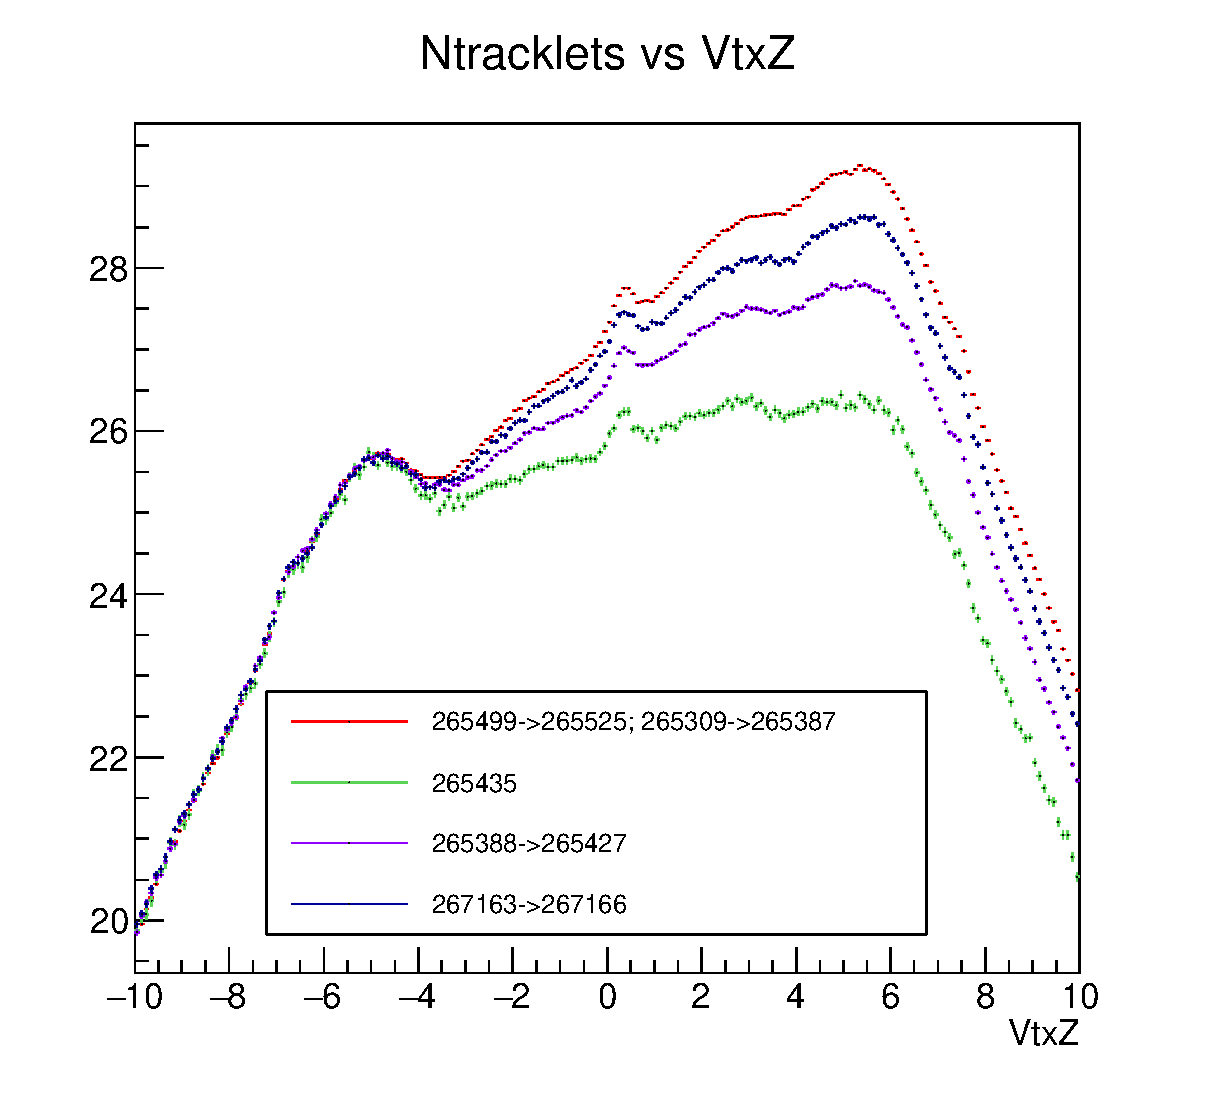
\includegraphics[width=.49\textwidth]{FigCap6/NtrkVsZVtx_FinalWeights.eps}
 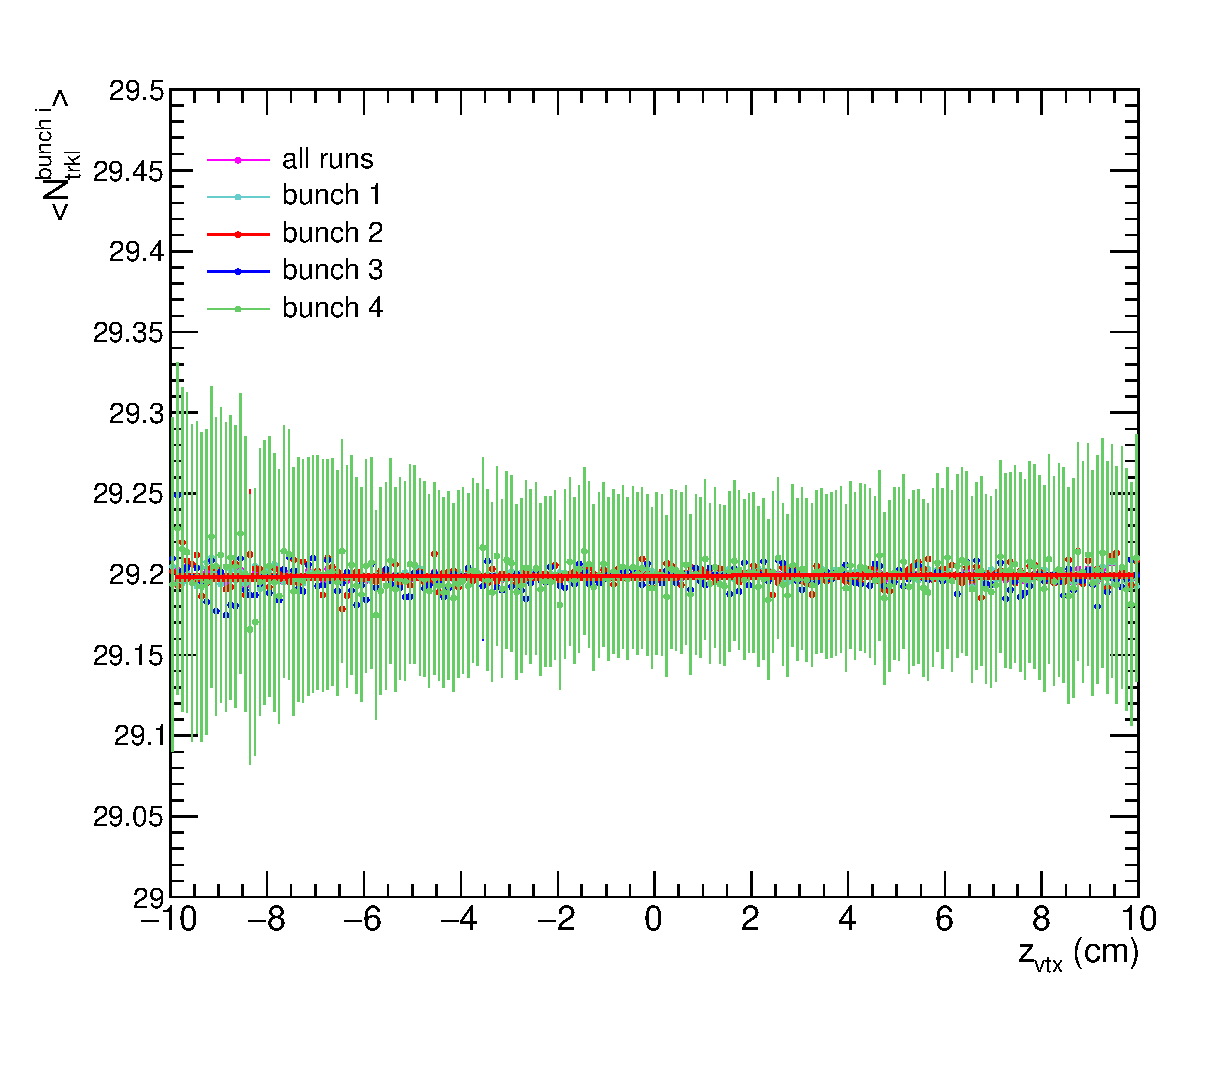
\includegraphics[width=.49\textwidth]{FigCap6/NtrkProfilesDataAfterZVxtEqual.eps}
 \caption{Left: average $\averNtrkl$ distributions as a function of $\zVtx$ for the four bunches of runs in different colours. Right: average $\averNtrkl$ distributions as a function of $\zVtx$ for the four bunches of runs in different colours, after the equalisation over $\zVtx$.}
 \label{fig:FourBunches}
\end{figure}

\section {Raw-yield extraction}
\label{sec:Rawyields_vs_mult}
The $\Ds$ signal was extracted in five $\pt$ intervals from 2 to 16 $\Gevc$, 
in three different classes of $N_{\rm trkl}$: $[1,40)$, $[40,70)$, $[70,200]$ tracklets.
The intervals were chosen in order to have sufficient statistics for the $\Ds$-meson yield extraction.
The same topological selections were used in the three multiplicity class in each $\pt$
interval and they were tuned to have good statistical significance of the extracted yields.
They are summarized in Tab.~\ref{tab:cutsDsVsNtrkl}.
\begin{table}[h!]
\centering
\begin{tabular}{|l|c|c|c|c|c|}
\hline
$\Ds$ topological selections & \multicolumn{5}{c|}{pt interval (GeV/$c$)}\\
\cline{2-6}
  & 2--4  & 4--6 & 6--8 & 8--12 & 12--16\\
\hline
Decay length ($\mum$)        & $>$300 & $>$350 & $>$350 & $>$400& $>$400\\
Decay length XY ($\mum$)     & $>$0 & $>$200 & $>$200 & $>$200 & $>$200\\
Norm Decay length XY          & $>$2.0& $>$0.0 & $>$2.0 & $>$2.0 & $>$2.0\\
Cosine pointing              & $>$0.94 & $>$0.95 & $>$0.95 & $>$0.97 & $>$0.97\\
$\sigma_{vertex}$  (cm)          & $<$0.02 & $<$0.03 & $<$0.03 & $<$0.06 & $<$0.06\\
$\Delta M$ (MeV/$c^{2}$) & $<$8.0 & $<$10.0 & $<$4.5 & $<$9.0 & $<$9.0\\
$\cos \theta^*(\pi)$    & $<$1.0 & $<$1.0 & $<$1.0 & $<$0.95 & $<$0.95\\
$|\cos^3 \theta^\prime({\rm K})|$        & $>$0.10 & $>$0.05 & $>$0.05 & $>$0.05 & $>$0.05\\
Norm. IP residual  & $<$2.5 & $<$2.0 & $<$2.0 & $<$2.0  & $<$2.0 \\
\hline
\end{tabular}
\caption{Topological selections used for the $\Ds$ meson in the five transverse momentum intervals consideredfor the three $N_{\rm trkl}$ classes.}
\label{tab:cutsDsVsNtrkl}
\end{table}
Fig.~\ref{fig:DsInvMassVsNtrkl_1},~\ref{fig:DsInvMassVsNtrkl_2} and~\ref{fig:DsInvMassVsNtrkl_3} 
show the invariant-mass fits performed in the five $\pt$ intervals, for the three 
multiplicity classes. The second peak on the left of $\Ds$ signal, around 1.88 MeV/$c^2$,
corresponds to $\Dplus$ decay contribution in the same channel considered of $\Ds$.
\begin{figure}[htpb]
\centering
 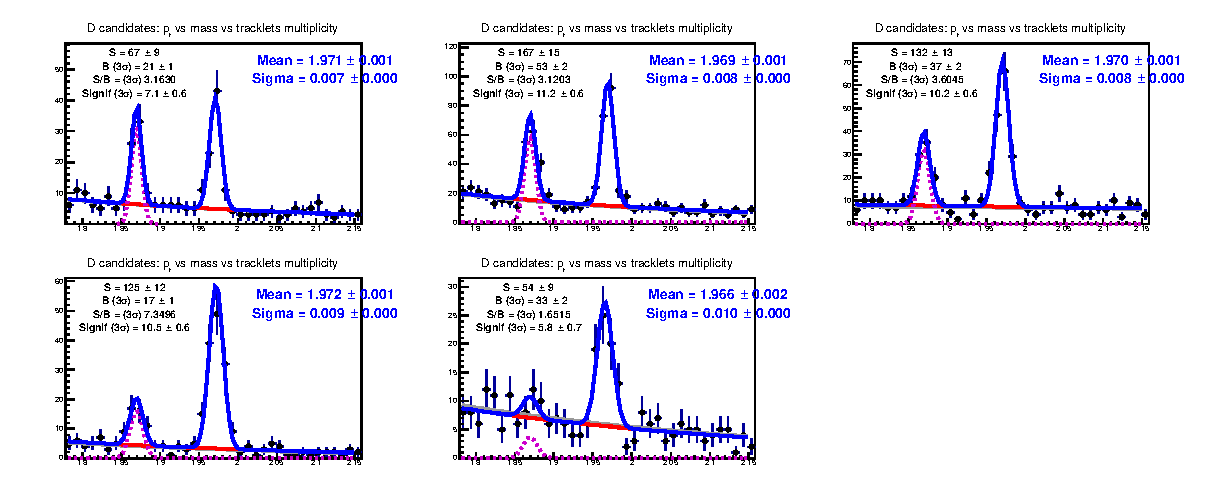
\includegraphics[width=.9\textwidth]{FigCap6/DsMass140.eps}
  \caption{$\Dsplus$ invariant-mass spectra, from 2 to 16 $\Gevc$, in the $1 \leq N_{\rm trkl} < 40$ interval.}
 \label{fig:DsInvMassVsNtrkl_1}
\end{figure}
\begin{figure}[htpb]
\centering
 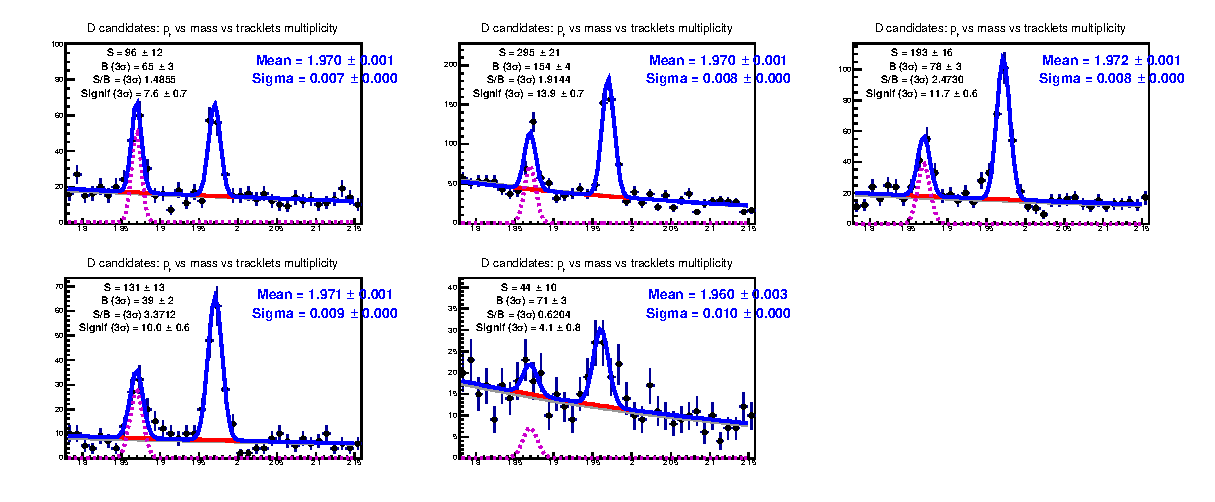
\includegraphics[width=.9\textwidth]{FigCap6/DsMass4070.eps}
  \caption{$\Dsplus$ invariant-mass spectra, from 2 to 16 $\Gevc$, in the $40 \leq N_{\rm trkl} < 70$ interval.}
 \label{fig:DsInvMassVsNtrkl_2}
\end{figure}
\begin{figure}[htpb]
\centering
 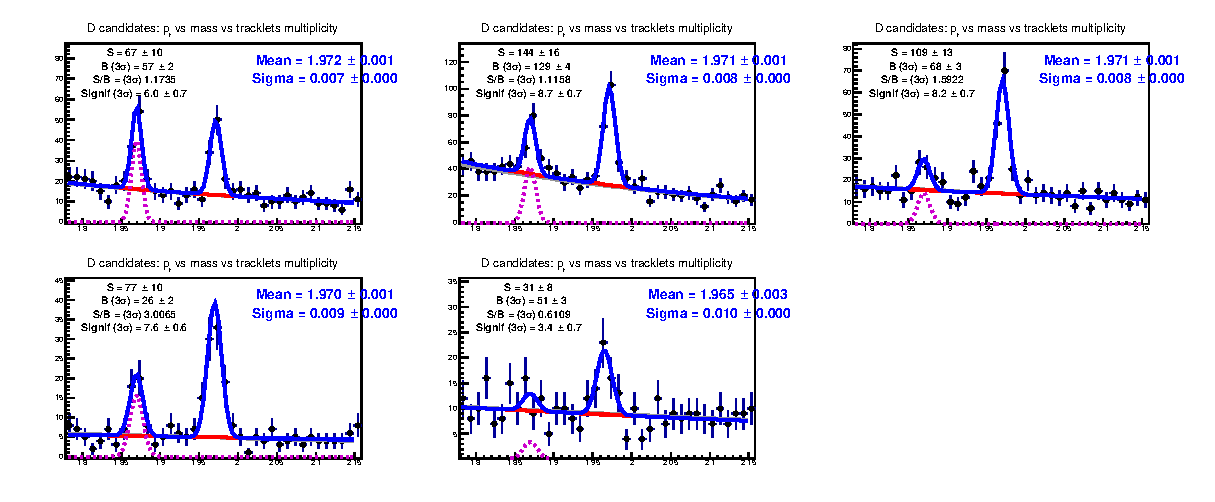
\includegraphics[width=.9\textwidth]{FigCap6/DsMass70200.eps}
  \caption{$\Dsplus$ invariant-mass spectra, from 2 to 16 $\Gevc$, in the $70 \leq N_{\rm trkl} \leq 200$ interval.}
 \label{fig:DsInvMassVsNtrkl_3}
\end{figure}
To avoid fluctuations, the $\Ds$ peak widths were fixed to the values obtained from the 
minimum-bias simulation (which were verified to be compatible to the values
from minimum-bias fit in data). In Fig.~\ref{fig:DsFitParamsVsNtrkl} 
the comparison of the Gaussian mean and width 
in data and minimum-bias MC is shown, as an example for the interval $40 \leq N_{\rm trkl} < 70$. 

\begin{figure}[htpb]
\centering
 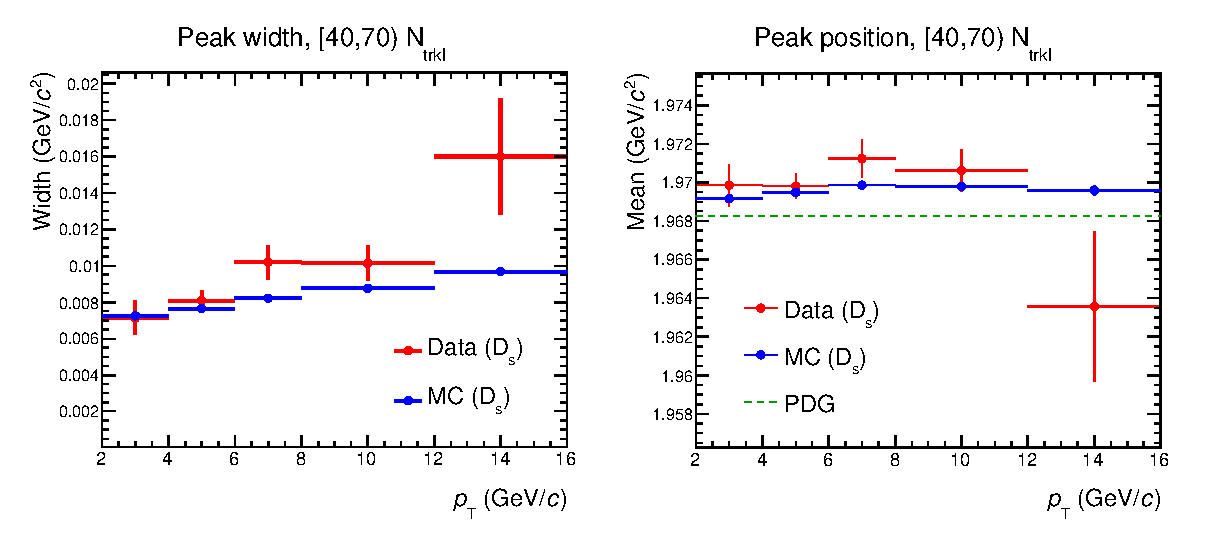
\includegraphics[width=.9\textwidth]{FigCap6/DsMeanSigma_DataMC_4070_Ntrkl.eps}
  \caption{$\Ds$ (and $\Dplus$ in the same $\Ds$ decay channel) peak width (left) and mean (right) obtained in the $N_{\rm trkl}$ intervals compared to the values from the data in the interval $40 \leq N_{\rm trkl} < 70$ and the minimum-bias MC simulation.}
 \label{fig:DsFitParamsVsNtrkl}
\end{figure}

\section{Corrections}
\label{sec:Corrections}
The $\Dsplus$/$\Dplus$ ratios in the multiplicity class $i$ were calculated
as:
\begin{equation} 
\label{eq:NtrklCorr}
 \frac{({\rm d}^2N_{\Ds}/{\rm d}\pt {\rm d}y)}{({\rm d}^2N_{\Dplus}/{\rm d}\pt {\rm d}y)} \Big |_i = \frac{Y^i_{\Ds}  f^i_{\rm prompt, \Ds} / ({\rm Acc} \times \epsilon)^i_{\rm prompt \Ds}}{Y^i_{\Dplus}  f^i_{\rm prompt, \Dplus} / ({\rm Acc} \times \epsilon)^i_{\rm prompt \Dplus}} \cdot \frac{\rm BR(\DstoKKpi)}{\rm BR(\DplustoKpipi)},
\end{equation}
where $Y$ is the extracted yield, which is corrected for the prompt fraction
$f_{\rm prompt}$, for the acceptance-times-efficiency term $({\rm Acc} \times \epsilon)$ and for
the branching ratio BR of the decay channel.\\



The acceptance-times-efficiency term was obtained via Monte Carlo simulations
using PYTHIA v6 with Perugia-2011 tuning as event generator and 
particles were transported through the detectors using GEANT3.
A $N_{coll}$ value is extracted for each PYTHIA event via a minimum-bias 
distribution obtained starting from a Glauber MC simulation. If the 
extracted number of binary collisions is larger than 1, a HIJING p-Pb 
event is added as the underlying event. 
Fig.~\ref{fig:NtrklDataMC} shows the distributions of $\Ntrkl$ in data and simulation,
after the equalisation over $\zVtx$, discussed in Sec.~\ref{sec:zVxtEq}. 
The selected events were required to have at least a $\Dzero$-meson candidate 
with the invariant mass compatible within 3$\sigma$ to the PDG $\Dzero$ mass. 
In order to not introduce differences in the multiplicity selection between data and MC, 
the distribution in the minimum-bias simulation needs to be corrected
with data-driven weights. From Fig.~\ref{fig:NtrklDataMC} one 
can notice that the simulated $\Ntrkl$ distribution reaches
lower values of $\Ntrkl$ with respect to data. It was checked 
that the selection efficiency of $\Ds$ is not dependent on
the tracklet multiplicity above 20 tracklets per event.
The correction factor was calculated independently for each of the 
four bunches of runs described in Sec.~\ref{sec:zVxtEq} (Fig.~\ref{Weights4Bunches}),
since also the inclusive distribution of the tracklets showed differences 
versus time related to the variation of the SPD configuration during the
period of data taking. In Fig.~\ref{fig:RatioNtrklMC} 
the ratio of the tracklet distributions for each of the four bunches
of runs to that obtained considering the full runlist is shown, to 
better clarify the necessity of four distinct corrections.
The resulting efficiency times acceptance factors are shown in 
Fig.~\ref{fig:DplusEffAccVsNtrkl} for the $\Dplus$ as a function of 
$N_{\rm trkl}$ and for the $\Ds$ as a function of $\pt$ are shown 
in Fig.~\ref{DplusEffAccVsNtrkl} and Fig.~\ref{DsEffAccVsNtrkl} 
respectively. As shown in these figures, the efficiency is almost flat 
as a function of the event multiplicity, and the largest difference is 
observed between the first $N_{\rm trkl}$ interval and the other two, as expected.


\begin{figure}[h]
\centering
 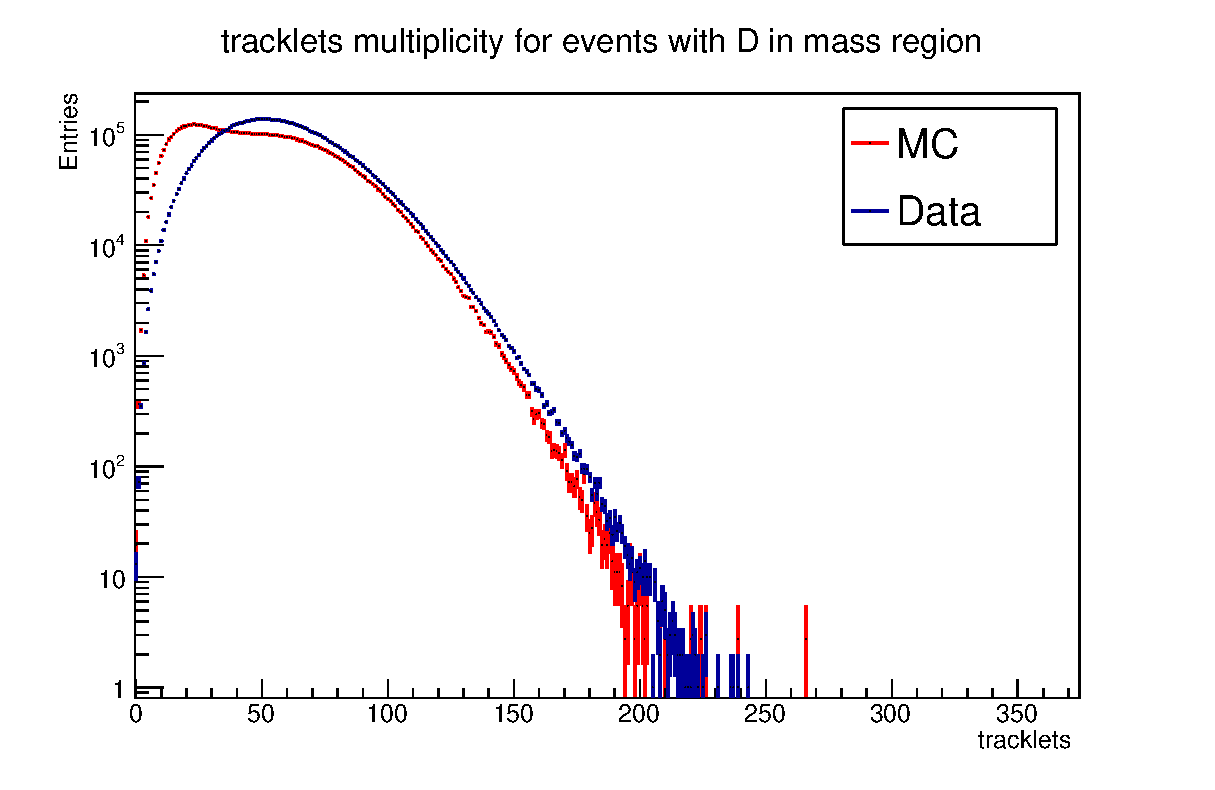
\includegraphics[width=.49\textwidth]{FigCap6/NtrkDistrWithDDataMC.eps}
 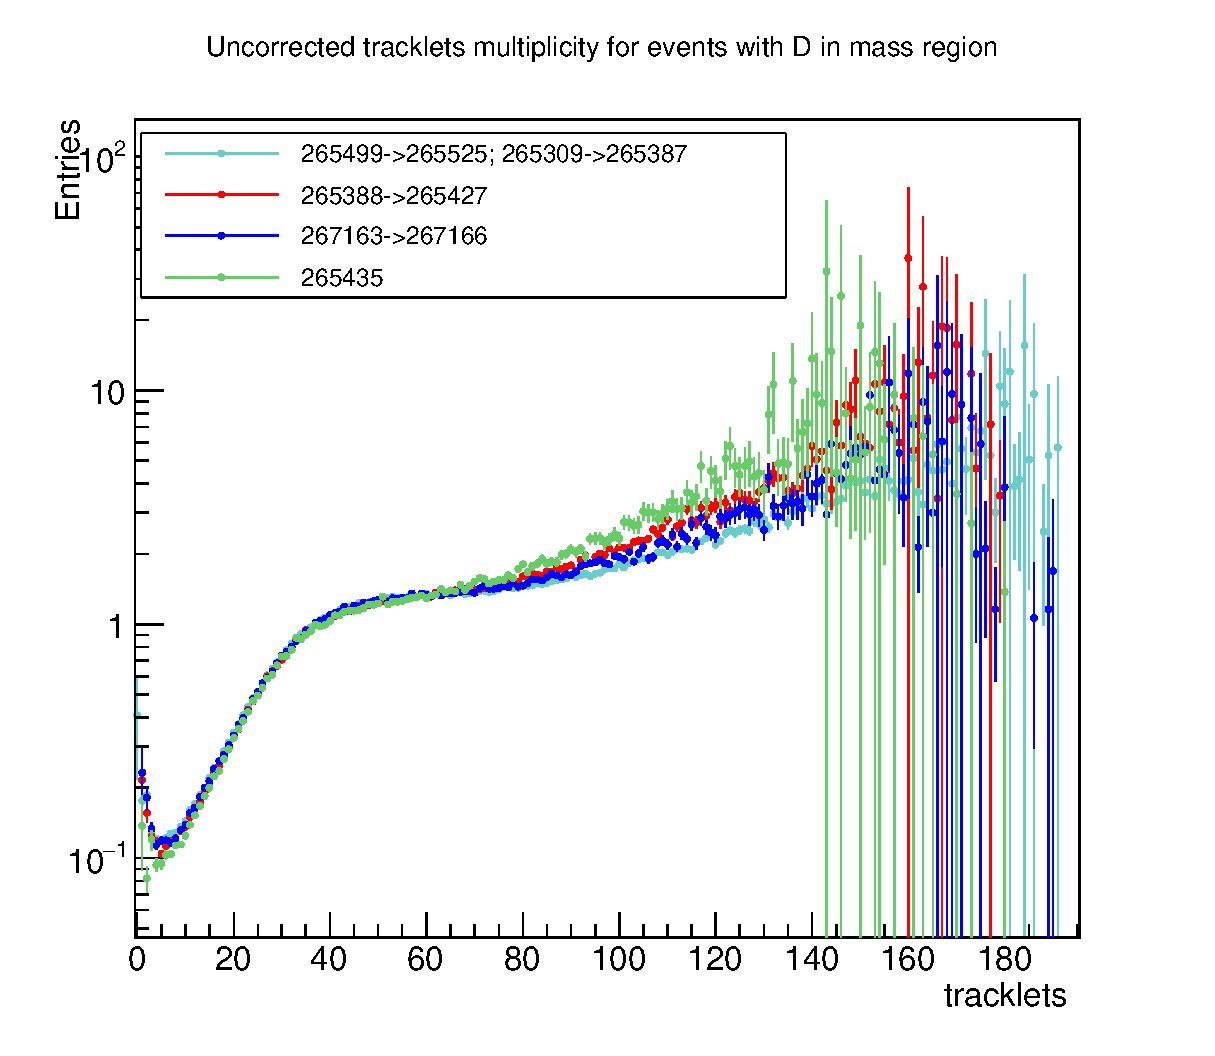
\includegraphics[width=.43\textwidth]{FigCap6/NtrklWeights4Bunches.eps}
 \caption{Left: tracklets distribution in data and in MC in different colours. Right: $\Ntrkl$-weight distributions for the MC in each of the four bunches of runs in different colours.}
 \label{fig:NtrklDataMC}
\end{figure}

\begin{figure}[h]
\centering
 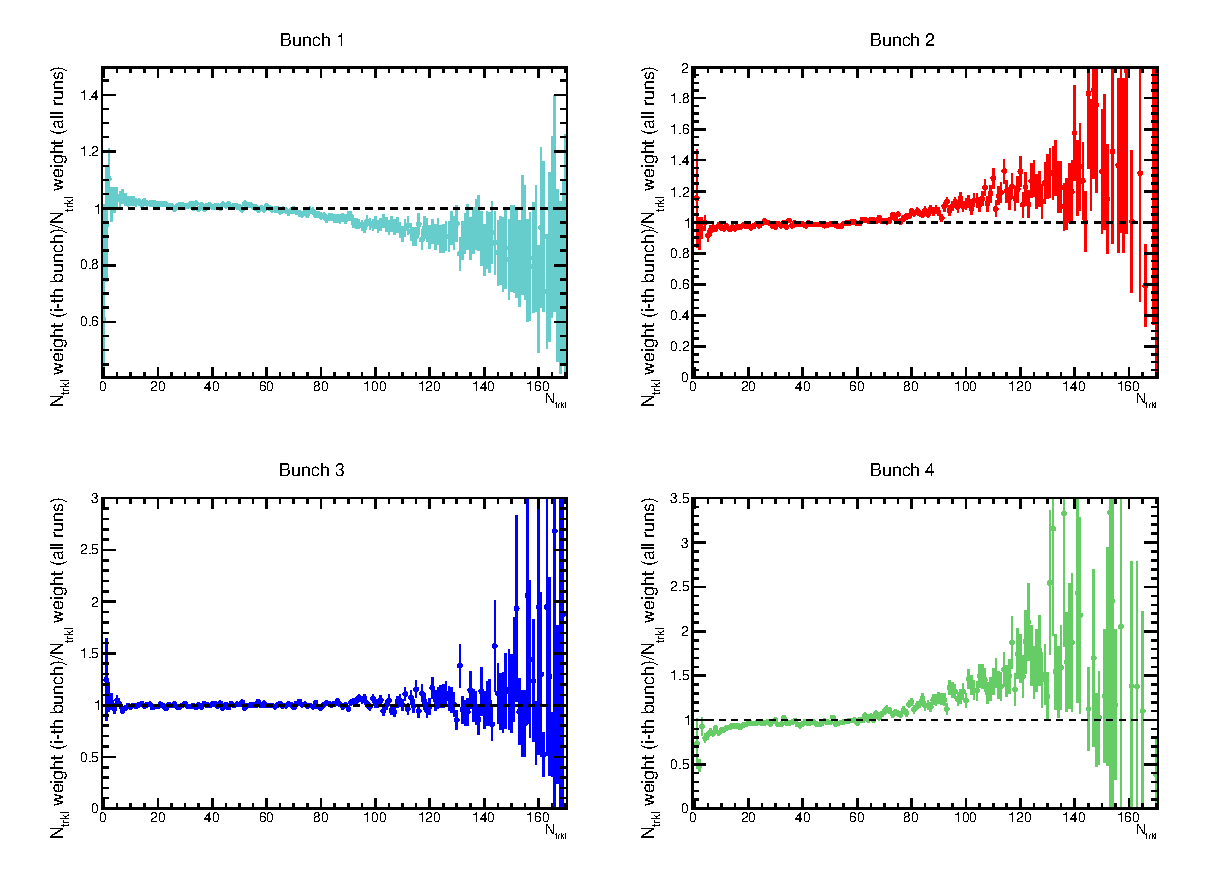
\includegraphics[width=.85\textwidth]{FigCap6/NtrkDistrMC_17d2a_EvWithD_zVxtUnCorr_896_897.eps}
 \caption{Ratio of the $\Ntrkl$ distribution for the MC in each of the four bunches of runs over the distribution obtained with the full statistics.}
 \label{fig:RatioNtrklMC}
\end{figure}

\begin{figure}[h]
\centering
 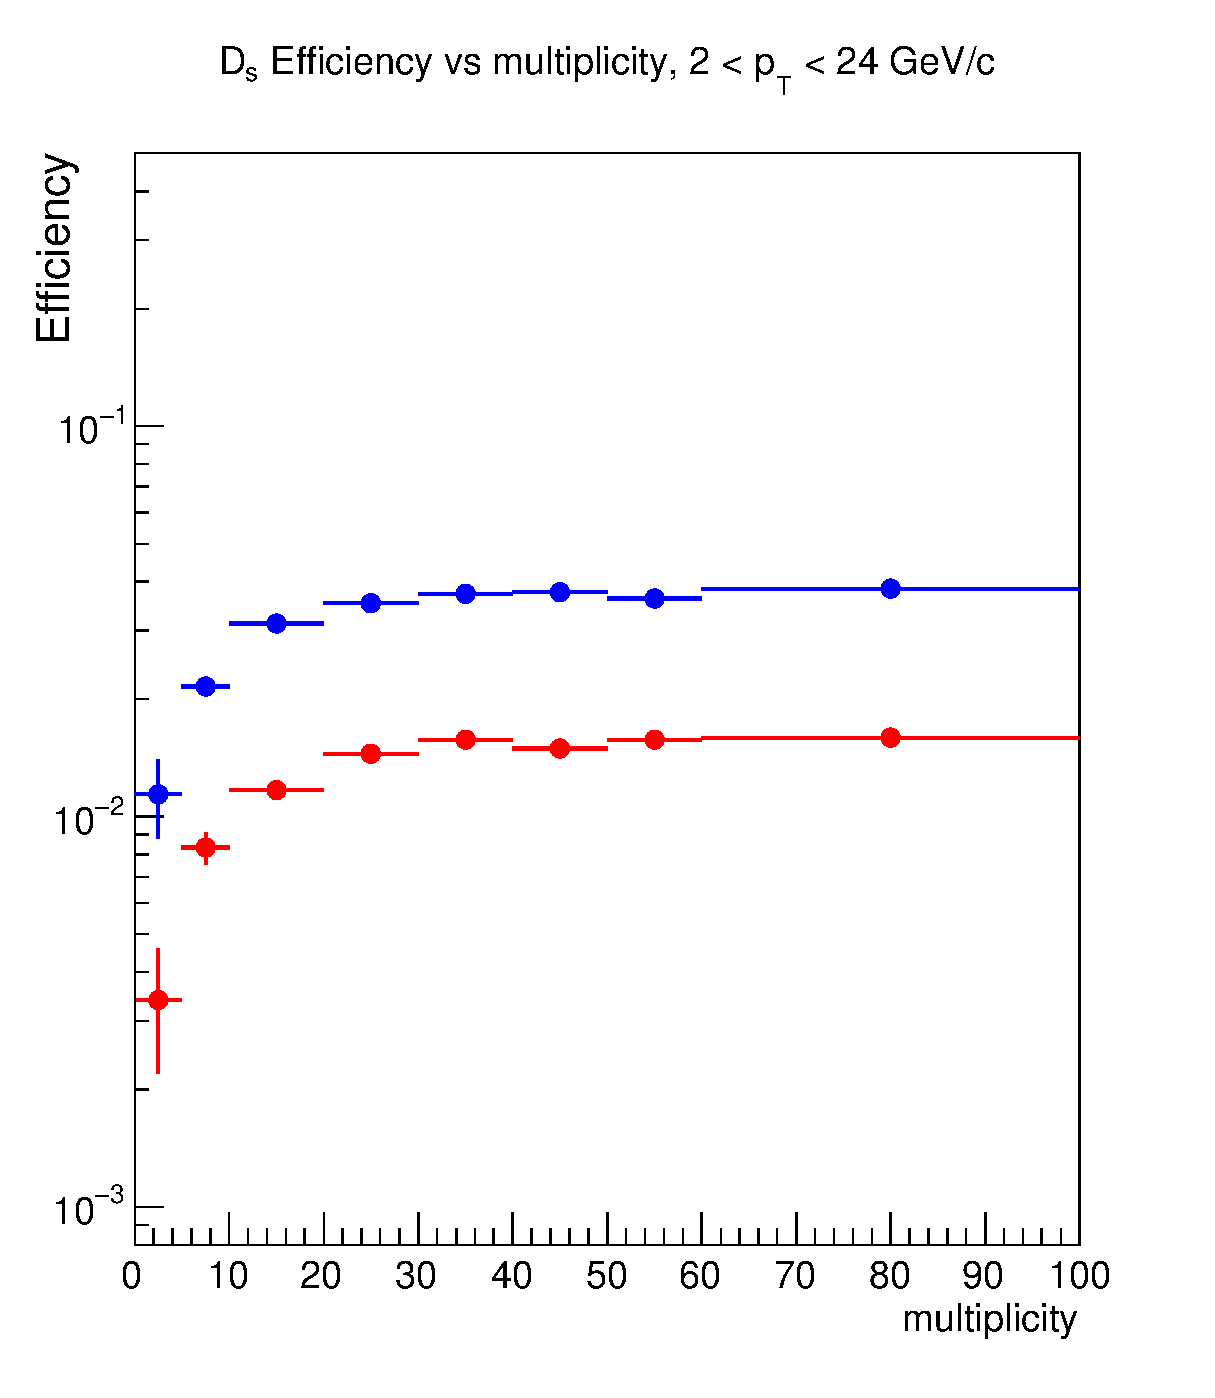
\includegraphics[width=.45\textwidth]{FigCap6/DsEffvsMult_pPb2016.eps}
 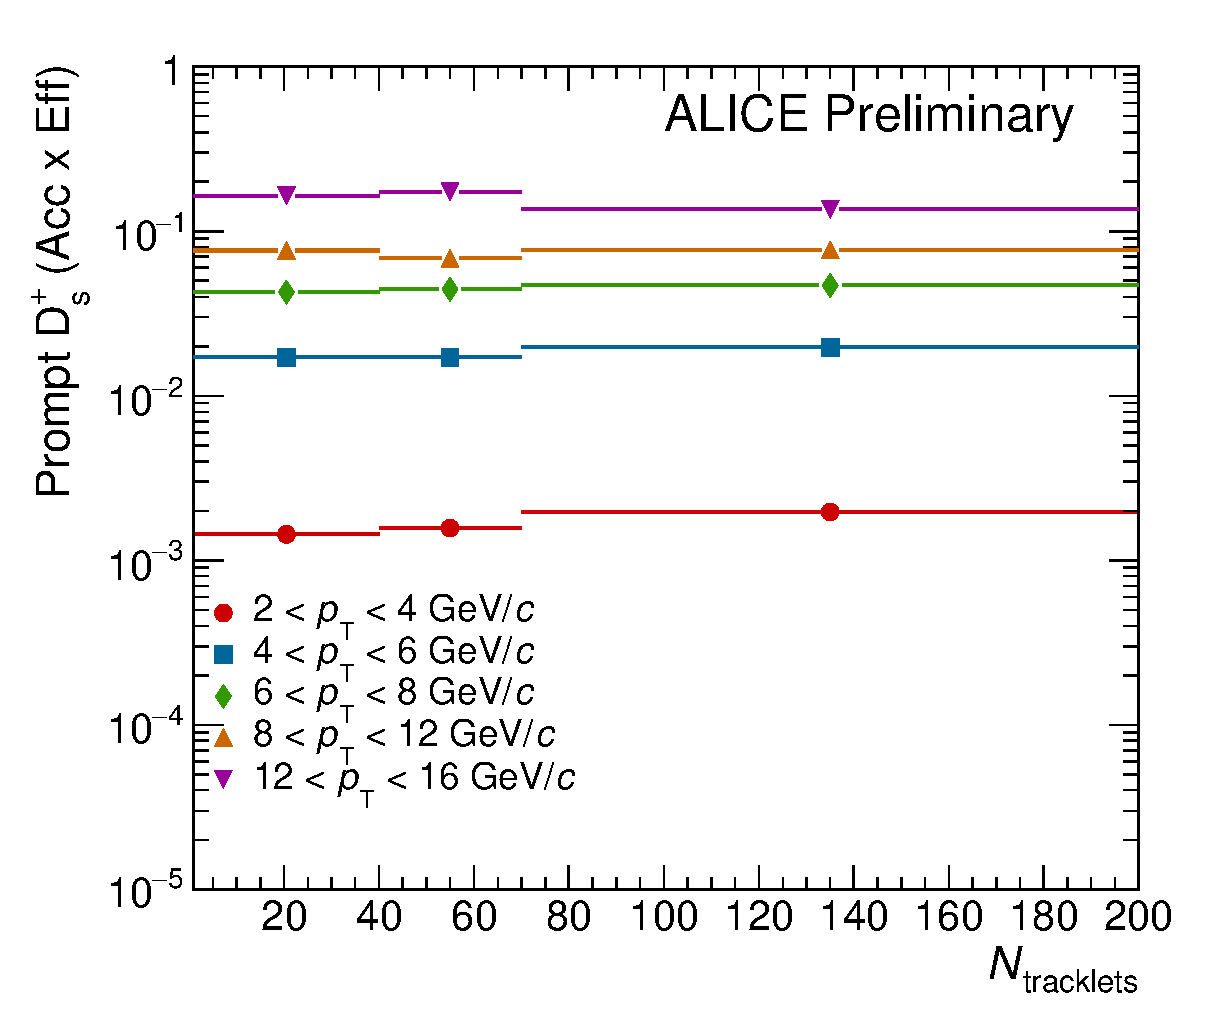
\includegraphics[width=.45\textwidth]{FigCap6/PromptDsEfficiency_times_Acceptance_VsNtrkl.eps}
 \caption{$\Ds$ efficiency as a function of the tracklet multiplicity, $\pt$-integrated between 2 and 24 $\Gevc$, in red for prompt and in blue for the feed-down.}
 \label{fig:DsEffVsMult}
\end{figure}



\subsection {Feed-down subtraction}
For the feed-down subtraction the FONLL-based method 
described in Sec~\ref{sec:FeedDown_Nb} was used. It was 
assumed that the fraction of prompt $\Ds$ (and $\Dplus$) does not depend on the 
multiplicity and therefore $f_{\rm prompt}$ was computed considering 
the minimum-bias sample for all the $N_{\rm trkl}$ classes. This hypothesis 
is also supported by the result obtained for the $\QpPb$ analysis, 
for which it was found that the fraction of prompt D is very similar 
in the two ZNA centrality classes and in the minimum bias sample 
(see Fig.~\ref{fig:DplusPromptFrac_010_60100}). A hypothesis on 
$R_{\rm pPb}^{\rm feed-down}$ is also needed, similarly to the Pb-Pb case in Eq.~\ref{eq:fprAA}.
It was assumed that $R_{\rm pPb}^{\rm feed-down} = R_{\rm pPb}^{\rm prompt}$ 
for both $\Ds$ and $\Dplus$, as done for the minimum-bias analysis~\ref{}. 
%This hypothesis was then varied between 
%$0.9 < R_{\rm pPb}^{\rm feed-down} = R_{\rm pPb}^{\rm prompt} <1.3$ 
%to estimate the systematic uncertainty, as will be described in more details in the dedicated section. 
In Fig~\ref{fig:DplusfPromptVsNtrkl} the fraction of prompt $\Dplus$ in the $\pt$ intervals of the analysis is shown.

\begin{figure}[htpb]
\centering
 \includegraphics[width=.7\textwidth]{FigCap6/DplusFprompt_Nb_d0cut_1_200.pdf}
  \caption{Fraction of prompt $\Dplus$ in the $\pt$ intervals considered for the analysis.}
 \label{fig:DplusfPromptVsNtrkl}
\end{figure}

\section {Systematic uncertainties}
\subsection{Raw-yield extraction}
\label{sec:rawYSystpA}
The systematic uncertainty due to the raw-yield extraction was 
estimated using the same strategy adopted in pp and Pb-Pb analyses. 
This approach is based on repeating many times the invariant-mass fit, 
combining in all the possible ways different fit configurations.
A distribution of the so-obtained yields is build, whose RMS is used as an 
estimator for the systematic uncertainty on the extraction.
Moreover, the results were compared to the values obtained with a bin 
counting method. The values assigned as systematic uncertainties are summarised 
in Tab.~\ref{tab:DsVsMult_syst}.

\subsection{MC $N_{\rm tracklets}$ distribution}
\label{sec:NtrkSyst}
Since the simulated $\Ntrkl$ distribution does not reproduce the multiplicity of the data, 
a correction was introduced to re-weight the D-meson efficiencies, as described 
in Sec.~\ref{sec:NtrklWeights_vsMult}. 
The distribution of $\Ntrkl$ obtained from the events that have at 
least a $\Dzero$ meson candidate, with no further request on the invariant mass,
was used to re-weight the $\Ds$ efficiencies and compare them with the one used for the central value.
In Fig.~\ref{fig:NtrklWeights_EvWithD_EvWithCand_Comparison} 
the comparison between the weights used as a default and those used 
to estimate a systematic uncertainty is shown for the four different 
bunches of runs (see Sec.~\ref{subsec:zVxtEq}).
Fig.~\ref{fig:DsDplusVsMult_SystEffWeights} shows the ratio between 
the efficiency re-weighted in this way to the default ones is shown. A 1\% uncertainty was assigned.

\begin{figure}[htpb]
\centering
 \includegraphics[width=.9\textwidth]{FigCap6/NtrkWeightsD-Cand_4Bunches_DsDplusVsmult.pdf}
 \caption{Comparison of the $\Ntrkl$ weights obtained from events with at least a $\Dzero$ candidate to those obtained from events with at least a $\Dzero$ candidate in the $\Dzero$ mass range (default).}
 \label{fig:NtrklWeights_EvWithD_EvWithCand_Comparison}
\end{figure}


\begin{figure}[htpb]
\centering
 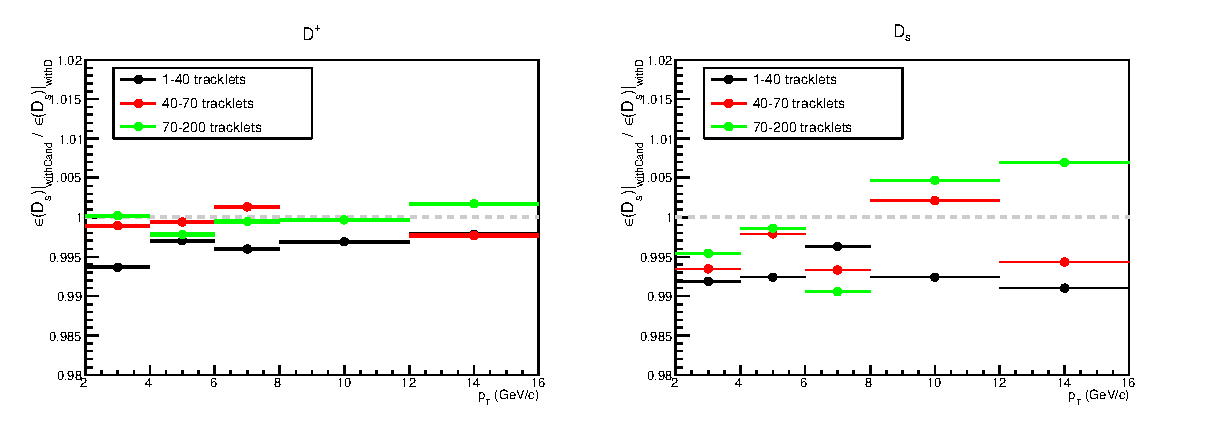
\includegraphics[width=.9\textwidth]{FigCap6/SystOnDWeightsWithCandVsWithD.eps}
 \caption{Ratio between the efficiency obtained with these weights, compared to the default ones, for $\Dplus$ (right) and $\Ds$ (left).}
 \label{fig:DsDplusVsMult_SystEffWeights}
\end{figure}

\subsection{Feed-down subtraction}
\label{sec:FDsyst}
The feed-down subtraction has been performed using the $N_{\rm b}$ 
method considering the full minimum-bias sample, assuming that the 
fraction of prompt D mesons was the same in the different $\Ntrkl$ 
classes of events. Also the systematic uncertainty on the prompt 
fraction is the same as the one evaluated for the minimum-bias sample. 
It comes from (i) the variation of the FONLL parameters (mainly from the 
renormalization scale) and (ii) the hypothesis on the $\RpPb$ of feed-down
 D mesons. In particular this hypothesis was varied in the range 
 $0.9 <\RpPb^{\rm feed-down}/\RpPb^{\rm prompt} < 1.3$.

\subsection{Topological selection efficiency}
\label{sec:CutVarsyst}
Since the D meson efficiency depends only slightly on the multiplicity 
(e.g. see Fig.~\ref{fig:DplusEffAccVsNtrkl}) and the same topological 
selections were applied in the different $\Ntrkl$ intervals, the systematic 
uncertainty was considered to be the same as the one estimated for the minimum-bias analysis.

\subsection{PID efficiency}
\label{sec:PIDsyst}
The PID efficiency is not expected to vary significantly with the 
multiplicity, and therefore the uncertainty on the PID selection efficiency 
was considered to be the same as the one estimated for the minimum-bias 
analysis. This is also supported by the study performed for the $\Dplus$
 in the two ZNA classes of events considered for the $\QpPb$ analysis (see Sec.\ref{sec:PIDsyst}).

\subsection{MC $\pt$ shape}
\label{sec:MCShapesyst}
As for the minimum-bias analysis also for the $\Ds/\Dplus$ as a function 
of multiplicity, the systematic uncertainty due to the MC $\pt$ shape was considered as negligible.

\subsection{Tracking efficiency}
\label{sec:TrackSyst}
The tracking efficiency is not expected to vary significantly with the 
multiplicity, and therefore the uncertainty on the tracking efficiency 
was considered to be the same as the one estimated for the minimum-bias analysis.

\subsection{Total systematic uncertainties}
\label{sec:Ratiosyst}
In Tab.~\ref{tab:DsVsMult_syst} the values of the systematic 
uncertainties for the $\Ds$ meson are summarized.
In the $\Ds/\Dplus$ ratio the following sources of systematic uncertainties were considered as uncorrelated:
\begin{itemize}
\item Raw-yield extraction
\item Topological selection efficiency
\item PID selection efficieny
\item MC $\pt$ shape (negligible)
\item Hypothesis on $\RpPb^{feed-down}$ for the feed-down D meson subtraction
\end{itemize} 
while
\begin{itemize}
\item MC $\Ntrkl$ distribution
\item Tracking efficiency
\item FONLL scale for the feed-down D meson subtraction
\end{itemize} 
as fully correlated.


\begin{table}[h!]
\centering
\scalebox{0.9}{
\begin{tabular}{|l|c|c|c|c|c|}
\hline
 $\Ds$ syst. unc. (\%) & \multicolumn{5}{c|}{$\pt$ interval ($\GeV/c$)}\\
\hline
 $1 \leq \Ntrkl < 40$ & 2--4  & 4--6 & 6--8 & 8--12 & 12--16 \\
\hline
Feed-down above &	3	& 3 &3 & 3	&5\\
Feed-down below &	4	&4 &4 &4 &5 \\
Cut variation & 14 & 9 & 8	& 8	&7\\
Raw yield  & 4 & 4 & 3 & 3 & 9\\
MC $\pt$-shape & negl & negl & negl & negl & negl \\
PID &  2 & 2 & 2 & 2 & 2 \\
Tracking & 4 & 4 & 4 & 4 & 4 \\
Multiplicity weights & 1 &  1 &  1 &  1 &  1 \\
\hline
 $40 \leq \Ntrkl < 70$ & 2--4  & 4--6 & 6--8 & 8--12 & 12--16 \\
\hline
Feed-down above &	3	& 3 &3 & 3	&5\\
Feed-down below &	4	&4 &4 &4 &5 \\
Cut variation & 14 & 9 & 8	& 8	&7\\
Raw yield  & 3 & 3 & 4 & 5 & 12\\
MC $\pt$-shape & negl & negl & negl & negl & negl \\
PID &  2 & 2 & 2 & 2 & 2 \\
Tracking & 4 & 4 & 4 & 4 & 4 \\
Multiplicity weights & 1 &  1 &  1 &  1 &  1 \\
\hline
 $70 \leq \Ntrkl < 200$ & 2--3  & 4--6 & 6--8 & 8--12 & 12--16 \\
\hline
Feed-down above &	3	& 3 &3 & 3	&5\\
Feed-down below &	4	&4 &4 &4 &5 \\
Cut variation & 14 & 9 & 8	& 8	&7\\
Raw yield  & 4 & 4 & 4 & 4 & 10\\
MC $\pt$-shape & negl & negl & negl & negl & negl \\
PID &  2 & 2 & 2 & 2 & 2 \\
Tracking & 4 & 4 & 4 & 4 & 4 \\
Multiplicity weights & 1 &  1 &  1 &  1 &  1 \\
\hline
\end{tabular}}
\caption{Systematic uncertainties on $\Ds$ for the $\Ds/\Dplus$ vs. multiplicity measurement.}
\label{tab:DsVsMult_syst}
\end{table}

\section {Conversion from tracklets to N charged particles}
\label{sec:NtrklToNch}
The conversion of the number of tracklets to the generated physical primaries ($\Nch$) 
was performed using the minimum-bias Monte Carlo production LHC17f2a (EPOS generator). 
The distribution of the measured $\Ntrkl$ as a function of the number of
$\Nch$ in the simulation was considered for this purpose, as shown in Fig.~\ref{fig:NtrklVsNch} left.
Physical primaries are defined as prompt particles produced in the collision and their
decay products, excluding those from weak decays of strange particles. The $z-$axis of
the 2D correlation was re-weighted with data-driven $\Ntrkl$ weights, to model the tracklet
distribution in the minimum bias production to that in data. 
The possible differences in the correlation
factor between tracklets and charged particles were eventually 
tested by comparing different generators (more details
in the systematics section). The proportionality factor was evaluated from a linear fit to the distribution, 
and was then applied to the mean $\Ntrkl$ value in each interval to estimate the $\averNch$ values. 
These values, shown in Fig.~\ref{fig:Nch} were then divided by the 
width of the considered $\eta$ range, $\Delta \eta =$ 2, 
to give an estimate of $\Nch$ per unit of pseudorapidity.

\begin{figure}[h]
\centering
 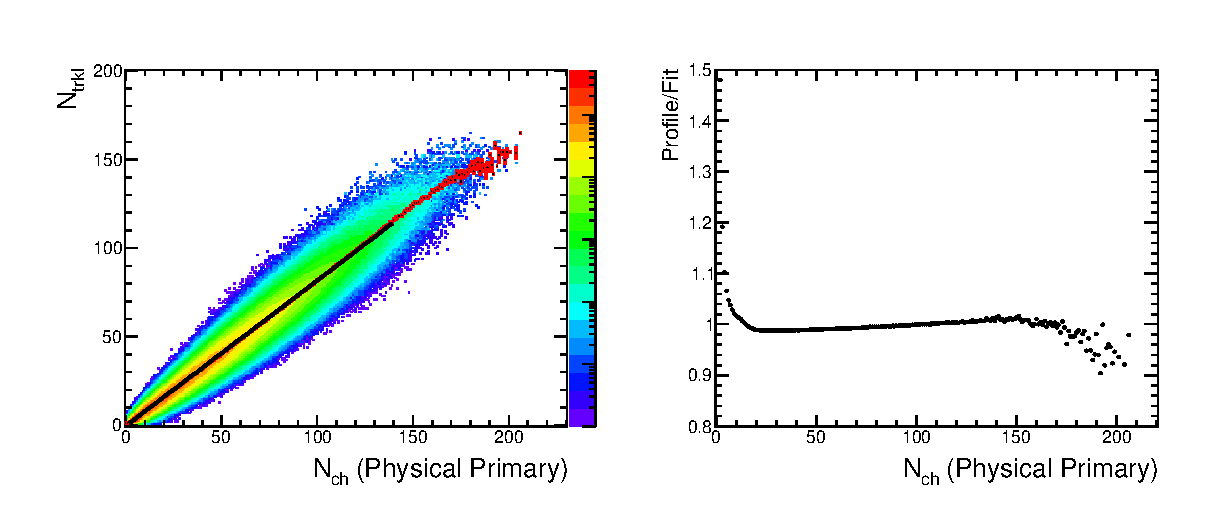
\includegraphics[width=1.\textwidth]{FigCap6/NtrklVsNchPhysPrimWithNtrklsReweight17f2a.eps}
 \caption{$\Ntrkl$ vs $\Nch$ distribution obtained for the 17f2a minimum bias production.}
 \label{fig:NtrklVsNch}
\end{figure}

\begin{figure}[h]
\centering
 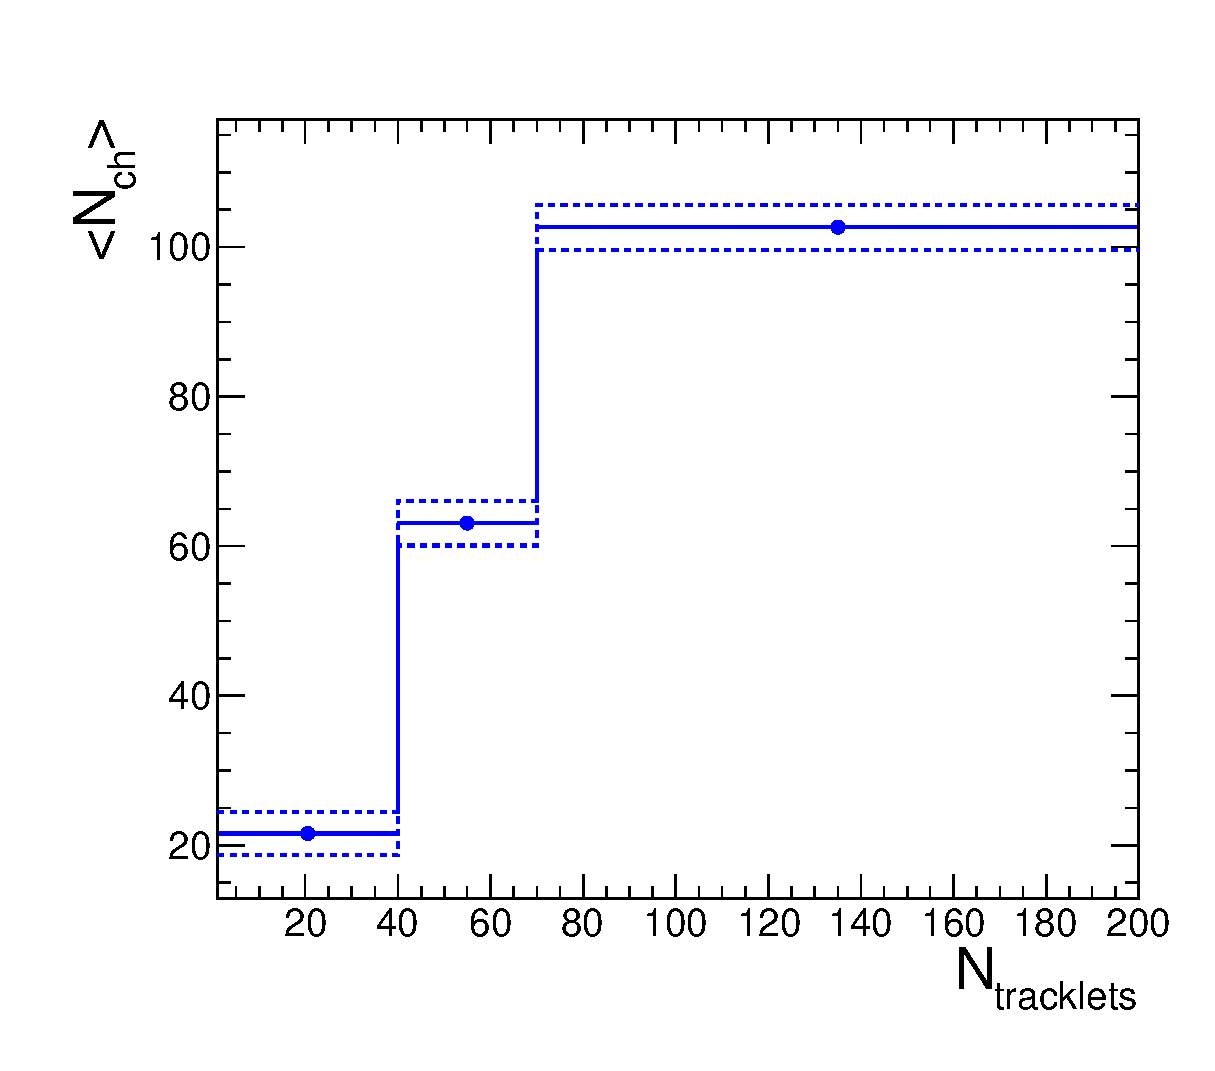
\includegraphics[width=.55\textwidth]{FigCap6/AverNchAndTotalSystUnc.eps}
 \caption{Average $\Nch$ values in the considered multiplicity classes, in the region $|\eta |< 1$. The lower and higher dashed lines represent the systematic uncertianties.}
 \label{fig:Nch}
\end{figure}

\subsection{Systematic uncertainty}
\label{sec:NtrklToNchSyst}
To estimate a systematic uncertainty on the evaluation of the average 
$\Nch$ value in the considered $\Ntrkl$ intervals, three different tests have been performed:
\begin{enumerate}
\item the conversion from $\Ntrkl$ to $\Nch$ was repeated with different MC generators 
\item the conversion from $\Ntrkl$ to $\Nch$ was repeated changing the 
assumption on the correlation (liear or not linear)
\item the conversion from $\Ntrkl$ to $\Nch$ was repeated with and without 
re-weighting the $\Ntrkl$ vs. $\Nch$ histogram with the data-driven $\Ntrkl$ weights
\end{enumerate}

In particular, for the first point, the procedure was repeated 
considering the minimum-bias Monte Carlo productions LHC17f2a 
(EPOS generator) and LHC17f2b (DPMJET generator). Moreover, 
the result was also compared to the one obtained using the charm 
and beauty enriched MC production LHC17d2a, however the last one 
was not taken into account for the systematic uncertainties, since the 
forced decays of injected particles could induce a bias in the number 
of charged particles at mid rapidity. Fig.~\ref{fig:NchVsMCgenerator} 
shows the comparison of the average $\Nch$ obtained from the different MC productions.

\begin{figure}[htpb]
\centering
 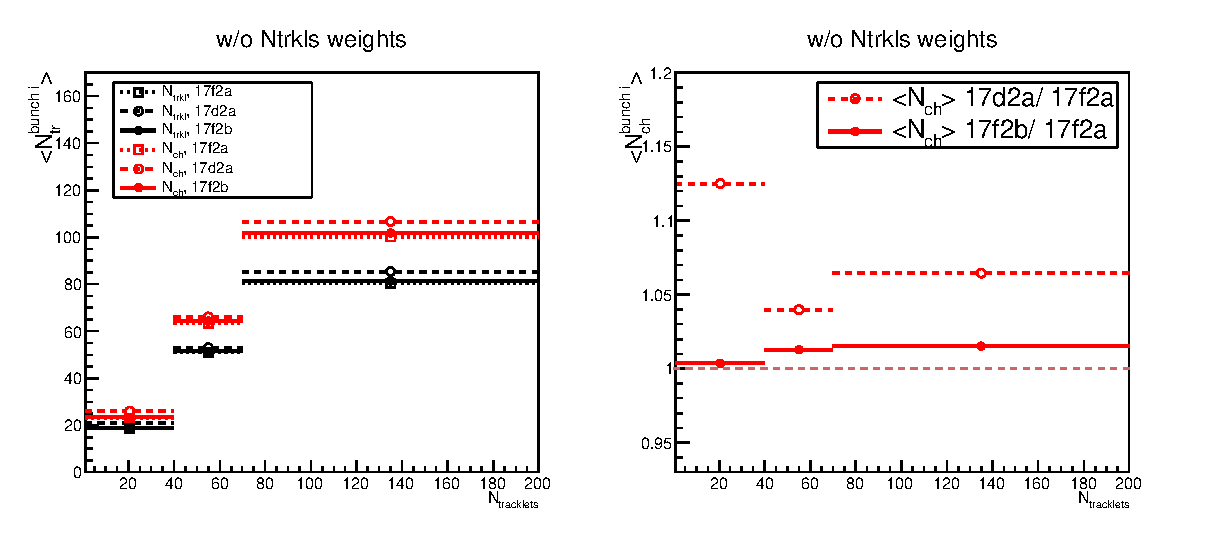
\includegraphics[width=.9\textwidth]{FigCap6/comparisonNtrkl_17f2b_17d2a_17f2a.eps}
 \caption{Left: Average $\Nch$ and $\Ntrkl$ values in the considered multiplicity classes, in the region $|\eta |< 1$, obtained from different MC productions. Right: ratio with respect to the default one (LHC172fa).}
 \label{fig:NchVsMCgenerator}
 \end{figure}

Considering the second source of uncertainty, the average $\Nch$ 
was extracted fitting the 2D histogram with a second order polynomial 
and considering the mean of the $\Nch$ distribution in the $\Ntrkl$ 
intervals considered in the analysis. This was done to test the possible 
non linear correlation between $\Ntrkl$ and $\Nch$, which is especially 
observed at low multiplicity, as shown in the right panel of Fig.~\ref{fig:NtrklVsNch}. 
In Fig.~\ref{fig:NchVsCorrHypo} the comparison of the average $\Nch$ 
obtained with the three different methods (linear fit, parabolic fit and mean of the $\Nch$ distribution) is shown.

\begin{figure}[htpb]
\centering
 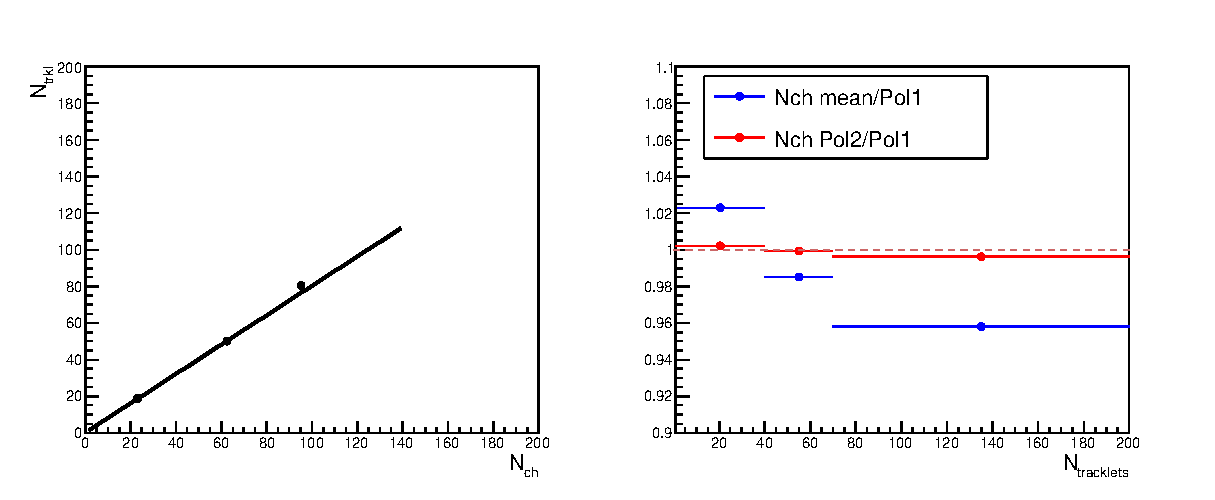
\includegraphics[width=.9\textwidth]{FigCap6/NchSystematics_linFit_17f2a}
 \caption{Comparison of the average $\Nch$ obtained with the three different methods (linear fit, parabolic fit and mean of the $\Nch$ distribution).}
 \label{fig:NchVsCorrHypo}
 \end{figure}

Finally, the average $\Nch$ was obtained without the data-driven 
$\Ntrkl$ weights and applying the weights obtained considering all 
the selected events, instead of the events that have at least a 
$\Dzero$ candidate in the correct mass range. This test is shown in Fig.~\ref{fig:NchVsNtrklWithWOweights}.

\begin{figure}[htpb]
\centering
 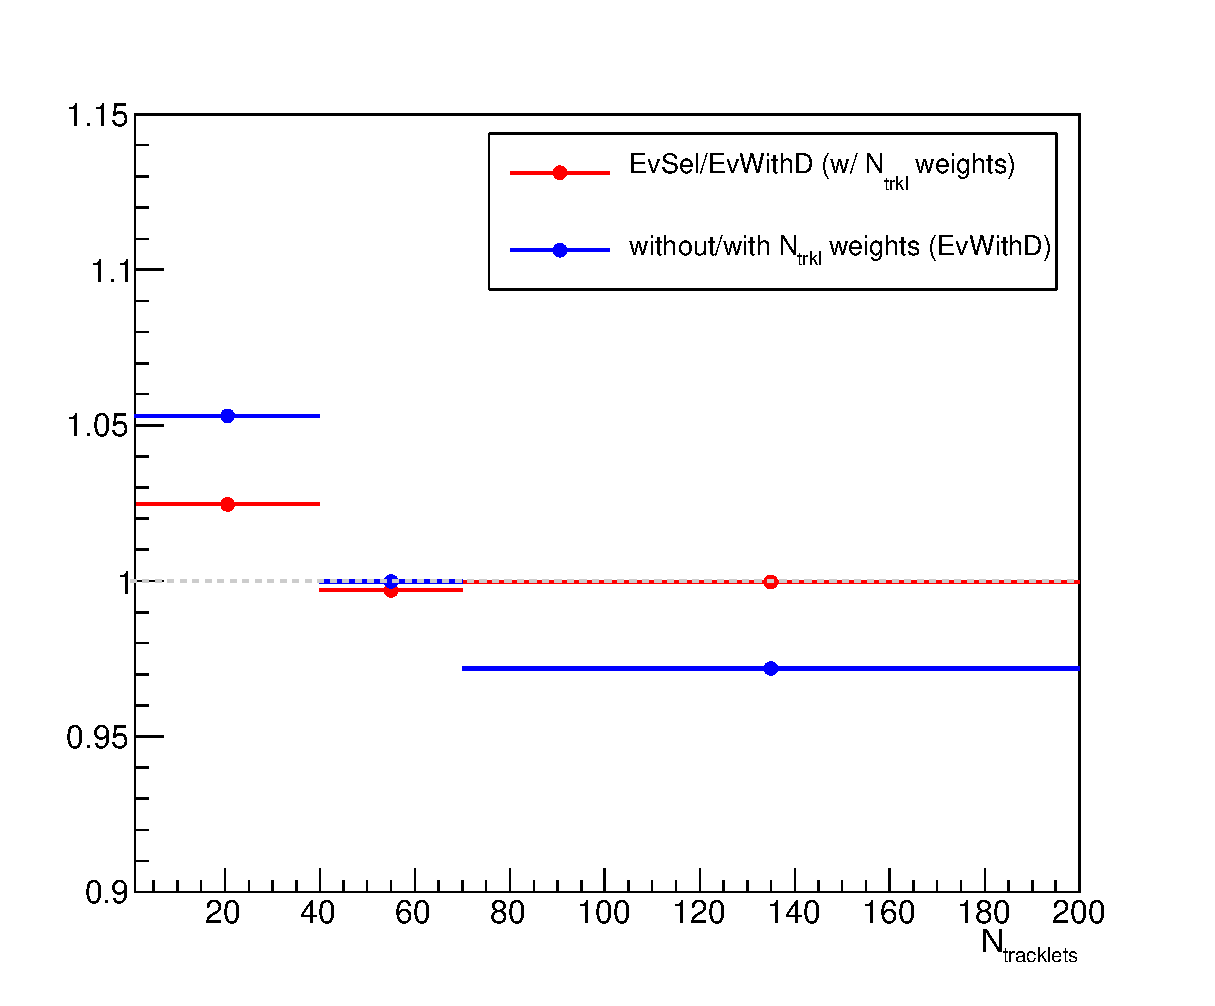
\includegraphics[width=.7\textwidth]{FigCap6/NchSystematics_NtrklWeights_17f2a.eps}
 \caption{Comparison of the average $\Nch$ obtained with and without data-driven $\Ntrkl$ weights.}
 \label{fig:NchVsNtrklWithWOweights}
 \end{figure}

Finally, the three sources of uncertainties have been considered as 
uncorrelated, and therefore summed in quadrature. The final result 
is shown in Fig.~\ref{fig:Nc}, where $\averNch$ in $|\eta|<1$ is shown 
with the corresponding systematic uncertainties.


\section{Results}
\label{sec:results}
The ratios of $\Ds/\Dplus$-meson yields are shown in Fig.~\ref{fig:DsDplusRatios} as a function of
the number of primary charged particles per unity of pseudo-rapidity, 
in the five $\pt$ intervals from 2 to 16 $\Gevc$.
The already measured ratios in pp collisions at $\sqrt{s}=$7 TeV and 
in Pb-Pb collisions at $\sqrt{s_{\rm NN}}=$ 5.02 TeV
(for the 0-10\%, 30-50\% and 60-100\% centrality classes, in the 
$\pt$ intervals where they are available) are also reported in the figure.
There is an hint of a non-flat trend between 2 $< \pt < 8~\Gevc$. The measured points were also
fitted with a linear function to have a quantitative indication of the slope, considering the statistical 
uncertainties only in the fit. The slopes from the linear fit on the pp, 
p-Pb and Pb-Pb points were found to be different from zero within 
1$\sigma$ of the parameter error between 2 $< \pt < 8 ~\Gevc$, and between 4 $< \pt < 8 ~\Gevc$ for the
fit on pp and p-Pb measurements only (Fig.~\ref{fig:FitRatios}).

\begin{figure}[h!]
    \begin{center}
          \includegraphics[width=0.9\textwidth]{./FigCap6/DsOverDplusVsMult_pp_pPb_PbPb.pdf}
    \end{center}
    \caption{ $\Ds/\Dplus$-meson yield ratios as a function of the primary charged particles in $|\eta|<0.5$, in the different $\pt$ intervals from 2 to 16 $\Gevc$.}
    \label{fig:DsDplusRatios}
\end{figure}

\begin{figure}[h!]
    \begin{center}
          \includegraphics[width=0.9\textwidth]{./FigCap6/Fit_DsOverDplusVsMult_pp7TeV_pPb5TeV_PbPb5TeV.pdf}
    \end{center}
    \caption{Linear fit on $\Ds/\Dplus$ ratios as a function of the primary charged particles, in the different $\pt$ intervals from 2 to 16 $\Gevc$. The slope of the pol1 is reported in each pad, for the fits made only on the pp and p--Pb measurements or on
    all the pp, p--Pb and Pb--Pb points.}
    \label{fig:FitRatios}
\end{figure}





